\scanpage{176}
\mspage{11}
% archive sheet number: 175
terminée si \deleted{nous prouvons que} \inserted{les $g_i(S)$} sont mutuellement disjointes et contenues dans l'ouvert de lissité de $\bar X$ sur $S$.
\deleted{\unsure{Il faut donc le} cas contraire, il faut examiner les ennuis qui peuvent se présenter : 1) \unsure{$g_i(s)$} $\exists i$ tel que $g_i(s)$ soit un pt double de $X_s$. Faisant éclater}

\figure{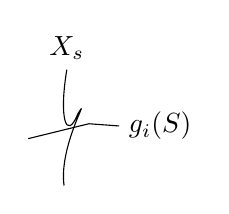
\begin{tikzpicture}[scale=.7]
\draw (0,-1) .. controls (-.1,-.3) and (.5,.7) .. (.25,.3)
.. controls (.05,-.2) and (-.1,.2) .. (.05,1.1);
\draw (-.65,-.15)--(.45,.12)--(1,.08);
\node[above] at (.05,1.1) {$X_s$};
\node[right] at (1,.08) {$g_i(S)$};
\end{tikzpicture}}

Mais si $D$ est le diviseur $X_s+\sum g_i(S)$ sur le schéma régulier $\bar X$, on sait (\quad) que, quitte à faire éclater un nb fini de fois des pts fermés de $\bar X$ (qui sont nécessairement dans $\bar X_s$, donc le processus ne touche pas à $\bar X_K$, \deleted{\unsure{ni}} à fortiori à $X_K$), on peut supposer que $D$ est à \uline{croisements normaux}. Mais ceci implique que les $g_i(S)$ sont mutuellement disjoints (sinon on aurait
\figure{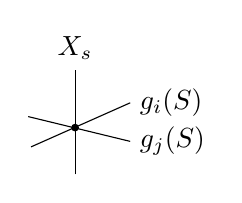
\begin{tikzpicture}[scale=.7]
\draw (0,-.8)--(0,1.1);
\draw (-.8,-.3)--(1,.5);
\draw (-.85,.25)--(1,-.2);
\fill (0,.05) circle (2pt);
\node[above] at (0,1.1) {$X_s$};
\node[right] at (1,.5) {$g_i(S)$};
\node[right] at (1,-.2) {$g_j(S)$};
\end{tikzpicture}}
, \deleted{\unsure{contraire}} qui n'est pas à croisements normaux).
\deleted{et que $g_i(S)\cap X_s=\{g_i(s)\}$ est un pt de lissité de $X_s$ (sinon on aurait}
\figure{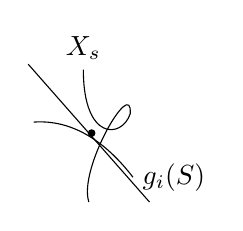
\begin{tikzpicture}[scale=.7]
\draw (0,-1) .. controls (-.2,-.4) and (.8,1.3) .. (.75,.6)
.. controls (.6,.15) and (-.1,.1) .. (-.1,1.4);
\draw (-1,.45) .. controls (-.3,.5) and (.3,.1) .. (.8,-.55);
\fill (.05,.25) circle (2pt);
\node[above] at (-.1,1.4) {\deleted{$X_s$}};
\node[right] at (.8,-.55) {\deleted{$g_i(S)$}};
\draw (-1.1,1.5)--(1.1,-1);
\end{tikzpicture}}
\deleted{). Enfin}
\inserted{D'autre part,} comme $X$ est \uline{régulier}, chaque section $g_i$ de $X$ sur $S$ est dans l'ouvert de lissité de $X$ (EGA IV 17\unsure{..}). La réduction de 1.3 au cas 1.4 est achevée.

\deleted{2.4. \uline{Réduction de 1.4 au cas de la dim. relative 1}, \unsure{projectif}}
\deleted{\unsure{prenons le} \illegible{2} \unsure{projectif} \illegible{2} de $S$ \illegible{2}}
\deleted{\inserted{Pour ceci, on peut supposer $X$ géom connexe de dim $n\geq2$} \unsure{Choisissons un} \illegible{1} et le th. prouvé en dim relative $<n$.}
\deleted{$\bar X\subset\mathbb P_S^r$, d'où $\bar X_s\subset P_s^r$. Soit $Z_s$ le normalisé de $\bar X_s$, de sorte qu'on a un morphisme \unsure{nat.|net}}
\[
\deleted{Z_s\longrightarrow P_s^r\quad\text{(EGA V)},}
\]
\deleted{$Z_s$ étant lisse \inserted{de dim $n$} \unsure{géométriquement}. On sait alors que pour un \deleted{\unsure{seul}} hyperpl ``assez général'' $H_s$ de $P_s^r$, $Z_s\mathbin{\times}_{\mathbb P_s^r}H=Z'_s$ est \unsure{connexe}}
